\subsubsection{方向导数与梯度}

\begin{definition}[Directional Derivative 方向导数]
    $$\lim_{t\to0}\frac{f(x+tv)-f(x)}{t}=\left.\frac{\partial f}{\partial v}\right|_x$$

    (if the limit exists)
\end{definition}

\emph{$\gamma_v(t)=x+tv$ special case $v=e_i$, $\frac{\partial f}{\partial e_i}=\frac{\partial f}{\partial x_i}$}

\begin{proposition}
    If $f$ is differentiable at $x$, then all derectional derivatives exist at $x$ and $\left.\frac{\partial f}{\partial v}\right|_x$ is linear in $v$, more precisely, $\left.\frac{\partial f}{\partial v}\right|_x = df|_x(v)$
    \begin{pf}
        $f(x+h)=f(x)+df|_x(h)+\circ(|h|)$, $h\to0$

        Restricting to the line $\gamma_v$ through $x$, we have $f(x_tv)=f(x)+df|_x(tv)+\circ(|tv|)$, $t\to0$

        $\implies\left.\frac{\partial f}{\partial v}\right|_x$ exists, and equal to $df|_x(v)$
    \end{pf}
\end{proposition}

Recall: $df|_x=\sum_{i=1}^n\frac{\partial f}{\partial x_i}(x)dx_i|_x$, i.e. $df|_x(v)=\sum_{i=1}^n\frac{\partial f}{\partial x_i}(x)v_i=\left<\nabla f|_x,v\right>$, $v=\sum_{i=1}^nv_ie_i$

\emph{$df(v)=\left<\nabla f,v\right>_{\mathbb{R}^n}$, $\nabla f\neq df$}

\begin{example}
    \begin{enumerate}
        \item $\begin{aligned}
                      x_i:     & \mathbb{R}^n\to\mathbb{R}    \\
                      dx_i|_x: & \begin{aligned}
                                     \mathbb{R}^n & \to\mathbb{R} \\
                                     v            & \mapsto v_i
                                 \end{aligned} \\
                  \end{aligned}$, $\nabla x_i|_x=e_i$\quad\raisebox{-0.5\height}{
\includegraphics[height=2cm]{chapters/09/02/0301}}\quad$\begin{aligned}
                      \text{gradient vector field} \\\text{梯度向量场}
                  \end{aligned}$
        \item $r=\sqrt{x^2+y^2},\theta=\arctan\frac{y}{x}$
              \begin{align*}
                  dr      & =\frac{x}{r}dx+\frac{y}{r}dy=\frac{x}{\sqrt{x^2+y^2}}dx+\frac{y}{\sqrt{x^2+y^2}}dy                        \\
                  d\theta & =\frac{-\frac{y}{x^2}}{1+\left(\frac{y}{x}\right)^2}dx+\frac{\frac{1}{x}}{1+\left(\frac{y}{x}\right)^2}dy \\
                          & =\frac{-y}{x^2+y^2}dx+\frac{x}{x^2+y^2}dy
              \end{align*}

              $\begin{aligned}
                       & |\nabla r|=1               & \nabla r|_{(x,y)}=\frac{x}{\sqrt{x^2+y^2}}\overrightarrow{i}+\frac{y}{\sqrt{x^2+y^2}}\overrightarrow{j} \\
                       & |\nabla\theta|=\frac{1}{r} & \nabla\theta=-\frac{y}{x^2+y^2}\overrightarrow{i}+\frac{x}{x^2+y^2}\overrightarrow{j}
                  \end{aligned}$\quad\raisebox{-0.5\height}{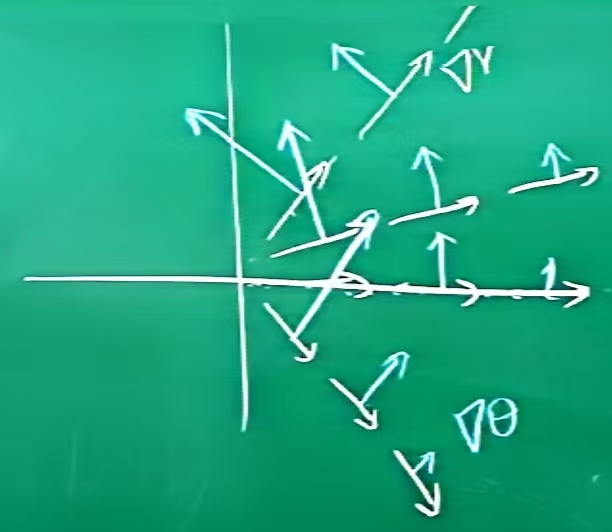
\includegraphics[height=2cm]{chapters/09/02/0302}}
    \end{enumerate}
\end{example}

$V$, $\mathbb{R}$ vector space

$V^*=\{\alpha\mid\alpha\text{ is a linear function on }V\}$

$\rightarrow(c_1\alpha+c_2\beta)(v)=c_1\alpha(v)+c_2\beta(v)$, $\forall v\in V$

$\implies c_1\alpha+c_2\beta$ is also linear

$\implies V$ is also naturally a vector space, \emph{called the ``dual space'' of $V$}

Suppose $(v_1,\dots,v_n)$ is a basis of $V$, then consider $\alpha_1,\dots,\alpha_n$ where $\alpha_i(v_j)=\delta_{ij}$

Claim: $\alpha_1,\dots,\alpha_n$ are independent
\begin{pf}
    Let $c_1\alpha_1+\dots+c_n\alpha_n=0$

    $\implies(c_1\alpha_1+\dots+c_n\alpha_n)(v_i)=C_i=0$, $\forall i=1,\dots,n$

    On the other hand, $\forall\alpha\in V^*$, $\alpha-\sum_{i=1}^n\alpha(v_i)\alpha_i\in V^*$

    $(\alpha-\sum_{i=1}^n\alpha(v_i)\alpha_i)(v_j)=\alpha(v_j)-\alpha(v_j)=0$, $\forall j=1,\dots,n$

    $\implies\alpha=\sum_{i=1}^n\alpha(v_i)\alpha_i$
\end{pf}

$f:\,\mathbb{R}^n=V\to\mathbb{R}$

$\Delta f=df|_x(\Delta x)+\circ(|\Delta x|)$

$df|_x\in V^*=\begin{aligned}
        df|_x                               & \mapsto\nabla f|_x=\nabla^{g_{E\cup C}} f \\
        (\mathbb{R}^n)^*                    & \simeq\mathbb{R}^n                        \\
        \left<\cdot,w\right>_{\mathbb{R}^n} & \mapsfrom w
    \end{aligned}$